\documentclass[12pt]{article}

\usepackage{geometry} 
\geometry{a4paper} 

\usepackage{graphicx}
\usepackage{CJK}
\usepackage{amssymb,amsmath,bm}
\usepackage{chngpage}
\usepackage{array}
\usepackage[noend]{algpseudocode}
\usepackage{algorithmicx,algorithm}
\usepackage{color}
\usepackage{mathrsfs}
\usepackage{longtable}
\usepackage{ltxtable, filecontents}
\usepackage{fancyhdr}    
\usepackage{lastpage}
\usepackage{float}

\pagestyle{fancy} %fancyhdr宏包新增的页面风格
\fancyhf{}
\rhead{Page \thepage\ of \pageref{LastPage}}%当前页  of 总页数

\begin{document}
\begin{CJK}{UTF8}{song}

\newcommand{\bN}{\mathbb{N}}
\newcommand{\tabincell}[2]{\begin{tabular}{@{}#1@{}}#2\end{tabular}}  

\title{金融服务计算\\项目文档}
\date{2017-12-27}
\author{作者:刘清仪,刘宏阳,李想,狄休,黄文瀚,廖超\\指导老师:英俊好,曹健}



\maketitle

\tableofcontents

%Chapter 1
\newpage
\section{项目简介}
\subsection{项目需求}
\begin{enumerate}
\item 实现一个能计算为现金流生成利率和贴现因子的利率模型。
\item 计算给定债券的到期现金流、股息和支付频率,计算债券价格、到期收益率、现值等指标。
\item 除了计算债券的现值、到期收益率,进一步计算债券的久期和凸性,以得到该债券对市场变动的敏感性程度。
\item 提供友好的用户界面。
\item 在上述系统分布式地、异步地部署在云端,并用百万级别的债券数据对系统的性能进行测试。
\end{enumerate}


\subsection{基本概念与定义}
Table\ref{tab:sys.param}给出了基本概念与定义。

\begin{filecontents}{mytable1.tex}
  \begin{longtable}{lX}
% 

    \hline
    名称 & 含义  \\ \hline
    Interest rate 利率 $r$& 利率,又叫利息率,是衡量利息高低的指标。是一定时期内利息额和本金的比率。利率=利息/本金。\\ \hline
    Discount factor 贴现因子 r &一般来说,当利率为r时,承诺T年之后支付R美元的现值是R美元/$(1+r)^T$。因此,即使没有通货膨胀,将来1美元的价值也小于现在1美元的价值,必须按某一数额贴现,该数额取决于利率的高低和收到货币的时间长短。其中$1/(1+r)^T$被称为未来T时期的货币的贴现因子. \\ \hline

    cash flow 现金流  &现金流量是现代理财学中的一个重要概念,是指企业在一定会计期间按现金收付实现制,通过一定经济活动(包括经营活动、投资活动、筹资活动和非经常性项目)而产生的现金流入、现金流出及其总量情况的总称。即:企业一定时期的现金和现金等价物的流入和流出的数量。\\ \hline
    Coupon 息票  & 息票一词来自英文coupon,原指旧时的债券票面的一部分,债券持有人可将其剪下,在债券付息日携至债券发行人处要求兑付当期利息。现在发行的债券多采用电子化形式,但票面利率(coupon rate)仍被用来表示债券的利率。\\ \hline
    Zero coupon bound 无息债券 & 无息债券 (Zero Coupon Bond) 债券无附设任何利息回报,发行机构以债券票面值在到期日偿还债券本金,故无息债券市价必定给予较票面值较大折让。 我国一次还本付息债券可视为无息债券.无息债券是指采用以复利计算的一次性付息方式付息的债券。无息债券又称“无息票债券”。按面值折扣发行,到期按面值十足还本的债券。\\ \hline

    Present Value 现值 $PV$ & 现值( Present value),指资金折算至基准年的数值,也称折现值、也称在用价值,是指对未来现金流量以恰当的折现率进行折现后的价值。指资产按照预计从其持续使用和最终处置中所产生的未来净现金流入量折现的金额,负债按照预计期限内需要偿还的未来净现金流出量折现的金额。\\ \hline
    Price 债券的市场价格  $P=v/{(1+y/f)^n} $& 债券在市场上交易时的价格。\\ \hline
    Face Value 票面价值  $v$& 债券面值是指债券发行时所设定的票面金额,它代表着发行人借入并承诺于未来债券到期日,偿付给债券持有人的金额。由于贴息债券的购买价低于债券面值,此外,债券发行有溢价发行和折价发行,因此,债券面值和投资债券的本金不一定相等。\\ \hline

    Yield 收益率 $y$ & 市场上同类债券的年化收益率,年化利率是通过产品的固有收益率折现到全年的利率。\\ \hline
    Payment Frequency 付息频率  $f$ & 一年支付利息次数。\\ \hline
    Time 付息次数  $n$& 累计计算利息次数。\\ \hline

    duration 久期 $D={dP/dy} \cdot {1/P}$ & 它是以未来时间发生的现金流,按照目前的收益率折现成现值,再用每笔现值乘以现在距离该笔现金流发生时间点的时间年限,然后进行求和,以这个总和除以债券目前的价格得到的数值就是久期。概括来说,就是债券各期现金流支付所需时间的加权平均值。\\ \hline
    convexity 凸性 $C={(d^2{P})/({dy}^2 )} \cdot {1/P}$& 久期描述了价格-收益率曲线的斜率,凸性描述了价格/收益率曲线的弯曲程度。凸性是债券价格对收益率的二阶导数。\\ \hline
 
  \caption{基本概念与定义}
  \label{tab:sys.param}
  \end{longtable}
\end{filecontents}
\LTXtable{\textwidth}{mytable1}

(备注:由于相同duration对不同金额的债券影响程度不一样,所以duration中除以了price,以进行规约化处理,convexity同理。)


 

%Chapter 2
\newpage
\section{计算模型及方法}
图\ref{fig:sys.param}给出了息票在市场上的价格P和市场上同类息票/债券的年化收益率y之间的定性关系。

\begin{figure}[htbp]
\begin{center}
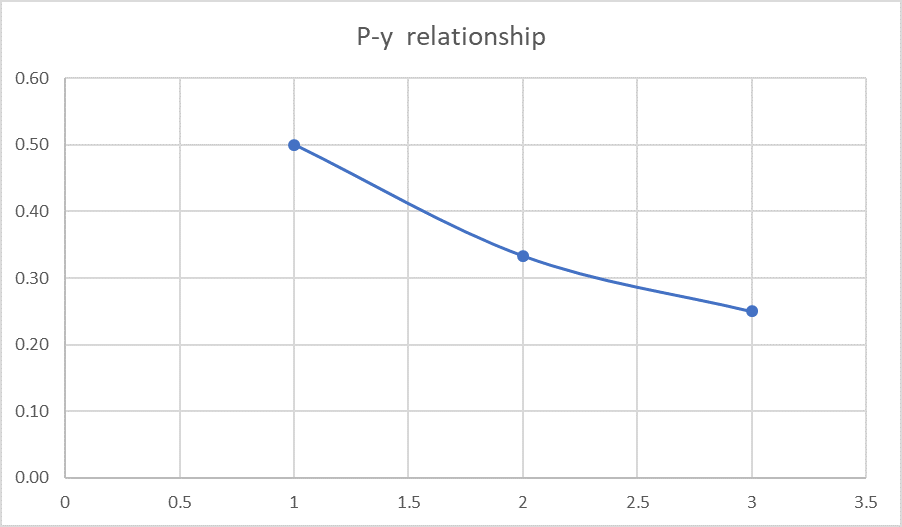
\includegraphics[width=16cm]{img//P_y_Relation.PNG}
\caption{P-y关系图}
\label{fig:sys.param}
\end{center}
\end{figure}

根据泰勒展开式

$P_1 \approx P_0-P_0 \cdot {Duration_D} \cdot (y_1-y_0 )+1/2 \cdot {P_0}\cdot {Convexity_D} \cdot (y_1-y_0 )$

这里的$Duration_D$和$Convexity_D$分别指的是一阶导数和二阶导数,没有除以Price。通过上式,我们可以通过当前息票价格求得未来某时刻息票价格。


%Chapter 3
\newpage
\section{系统数据架构}
\subsection{开发环境}
开发环境包括编程语言、软件环境、硬件环境等。
\begin{table}[H]
\begin{adjustwidth}{-3cm}{-3cm}
\begin{center}
\begin{tabular}{|p{.2\textwidth}| p{.8\textwidth}|} \hline
计算逻辑 & Python2.7  \\ \hline
前端框架 & Flask  \\ \hline
前端展示 & HTML5  \\ \hline
数据库 & MySQL \\ \hline

系统 & Ubuntu 16.04.3 LTS  \\ \hline

处理器 & Ubuntu Intel Core5  \\ \hline
\end{tabular}
\end{center}
\end{adjustwidth}
\end{table}



\subsection{数据来源}
\begin{itemize}
\item 国泰安CSMAR数据库专注于学术高校研究

\item 覆盖经济、股票、基金、债券等领域,涵盖面广。

\item 数据做深层衍生加工,而CSMAR侧重于数据的深度,强调对原始数据的深层专业加工、整理,属精准数据。

\item CSMAR支持EXCEL、TXT、XML、 SAS 、STATA 、MATLAB 、R等多种格式。

\end{itemize}

\subsection{数据结构}
本系统使用了352万条数据,以进行大数据情况下的系统性能测试。
\begin{table}[H]
\begin{adjustwidth}{-3cm}{-3cm}
\begin{center}
\begin{tabular}{|p{.3\textwidth}| p{.7\textwidth}|} \hline
债券基本情况表 & 据总记录数:104949,记录区间:1990-2017  \\ \hline
债券日交易信息表 & 数据总记录数:3524198,数据开始时间:1996-2017
存储债券每日交易信息,包括价格,成交量,涨跌幅等
 \\ \hline
\end{tabular}
\end{center}
\end{adjustwidth}
\end{table}

Figure \ref{fig:sys.param}为数据结构示意图。
\begin{figure}[H]
\begin{center}
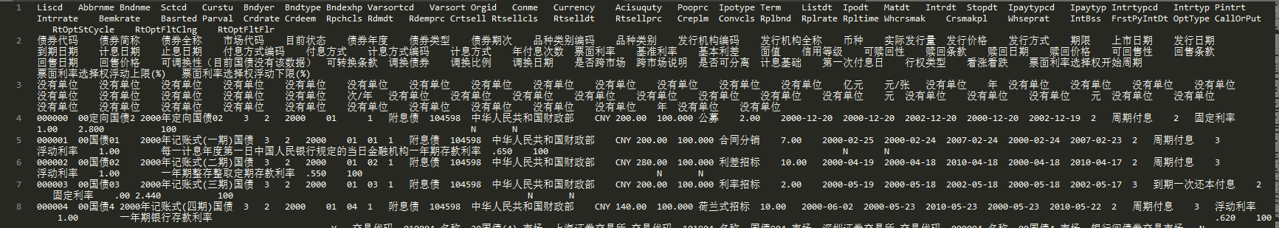
\includegraphics[width=16cm]{img//DataStructure.PNG}
\caption{数据结构示意图}
\label{fig:sys.param}
\end{center}
\end{figure}



\subsection{数据库设计}
本系统使用MySQL数据库。
\begin{table}[H]
\begin{adjustwidth}{-3cm}{-3cm}
\begin{center}
\begin{tabular}{|p{.3\textwidth}| p{.7\textwidth}|} \hline
债券基本情况表 & 主键:债券id  \\ \hline
债券日交易信息表 & 主键:债券id+交易日期\\ \hline
\end{tabular}
\end{center}
\end{adjustwidth}
\end{table}


\subsection{数据库性能}
我们测试了数据库在不同情况下的处理速度。
\begin{table}[H]
\begin{adjustwidth}{-3cm}{-3cm}
\begin{center}
\begin{tabular}{|p{.3\textwidth}| p{.7\textwidth}|} \hline
实验目的 & 测试数据库对大量请求响应的处理速度  \\ \hline
实验过程 &给出10000个(债券id,交易时间),由数据库取出最相似的交易信息\\ \hline
\end{tabular}
\end{center}
\end{adjustwidth}
\end{table}

Figure \ref{fig:sys.param}为使用全Varchar字段情况。
\begin{figure}[H]
\begin{center}
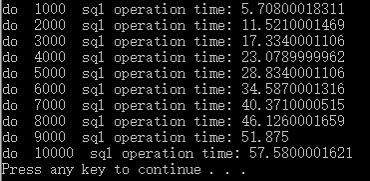
\includegraphics[width=16cm]{img//Varchar.PNG}
\caption{使用全Varchar字段情况}
\label{fig:sys.param}
\end{center}
\end{figure}

Figure \ref{fig:sys.param}为使用int类型和data类型情况。
\begin{figure}[H]
\begin{center}
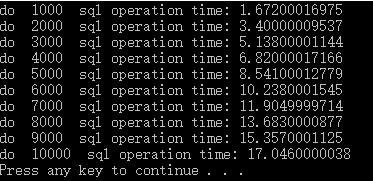
\includegraphics[width=16cm]{img//int_data.PNG}
\caption{使用int类型和data类型情况}
\label{fig:sys.param}
\end{center}
\end{figure}

Figure \ref{fig:sys.param}为多个query组合情况。
\begin{figure}[H]
\begin{center}
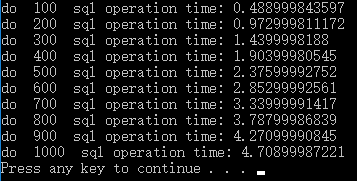
\includegraphics[width=16cm]{img//multi_query.PNG}
\caption{多个query组合情况}
\label{fig:sys.param}
\end{center}
\end{figure}

Figure \ref{fig:sys.param}为不同情况下数据库性能比较。
\begin{figure}[H]
\begin{center}
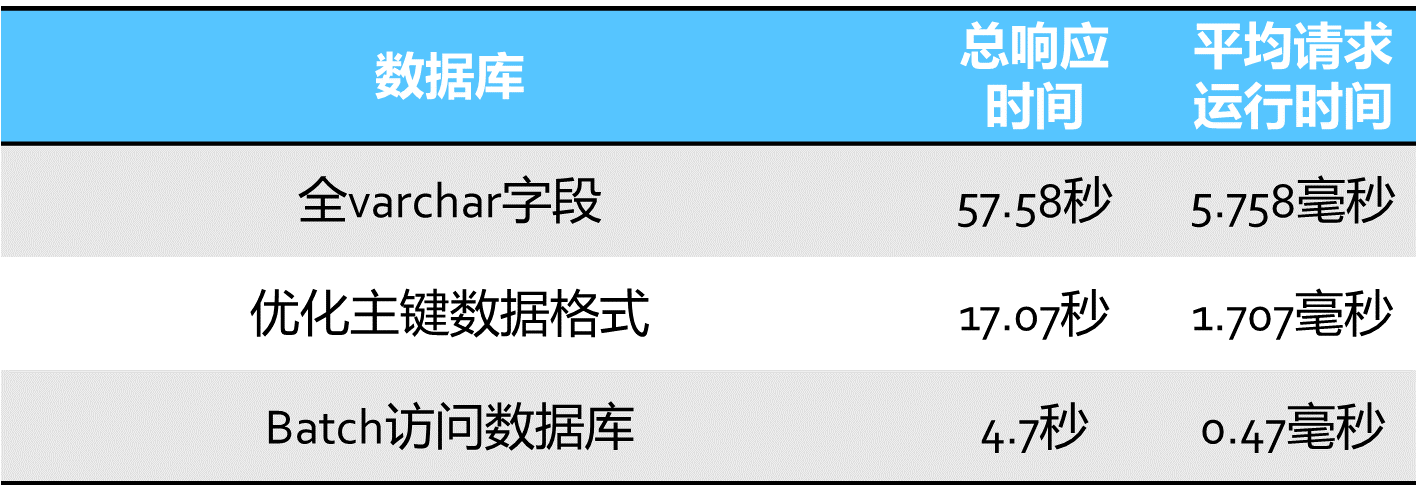
\includegraphics[width=16cm]{img//DB_performance.PNG}
\caption{不同情况下数据库性能比较}
\label{fig:sys.param}
\end{center}
\end{figure}

\subsection{数据测试集}
为了对该系统的性能进行测试,我们模拟生成了100万条债券数据。数据格式为json格式,包括6项数据:
\begin{enumerate}
\item 发行时间
\item 年限
\item 付息频率
\item 面值
\item 付息利率
\item 出售时间
\end{enumerate}

Figure \ref{fig:sys.param}为数据的Json格式。
\begin{figure}[H]
\begin{center}
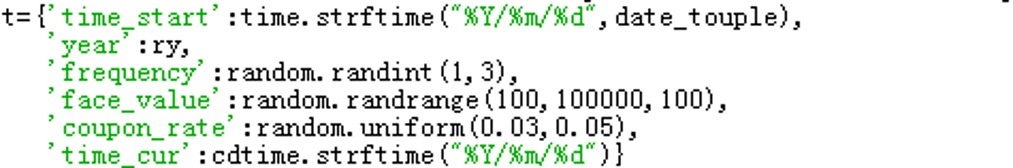
\includegraphics[width=16cm]{img//test_data.PNG}
\caption{数据的Json格式}
\label{fig:sys.param}
\end{center}
\end{figure}

%Chapter 4
\newpage
\section{系统模块划分}
图\ref{fig:sys.param}给出了Dirty Price与时间t的关系。
\begin{figure}[htbp]
\begin{center}
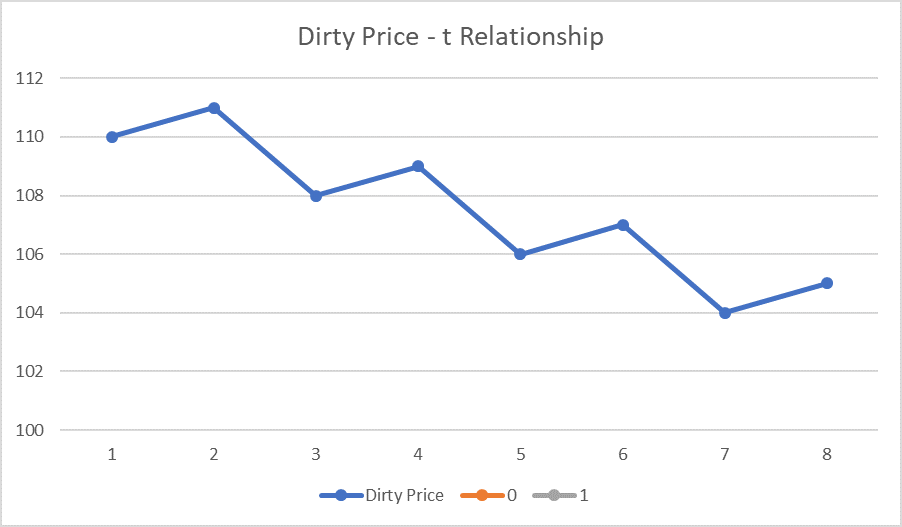
\includegraphics[width=16cm]{img//DirPri_t_Relation.PNG}
\caption{Dirty Price与时间t的关系}
\label{fig:sys.param}
\end{center}
\end{figure}

Dirty price指的是clean price和accrued interest(已经发放的利息)的和。
Clean price指的是还未领取的息票本金折现到当前时刻是多少钱。

其中t坐标轴的偶数(2,4,6,8,……)指的是股息发放日。每次发放股息后,coupon的dirty price等于clean price。随着利息的积累,dirty price逐渐高于clean price,直到下次股息发放日股息再次方法,dirty price再次等于clean price。
市场上的报价通常是clean price,所以交易双方需要根据自己的交易模型计算出accrued interest,在交易时把积累的利息加上去。

对于Duration和convexity,我们有以下结论:
1.Duration的加权平均就是该coupon bond的加权平均
2.Convexity 的加权平均就是该coupon bond的加权平均

规范化表示:
$Duration_avg=(P*V_1*D_1+P*V_2*D_2+ \cdots)/(P*V_1+P*V_2+\cdots)$
$Convexity_avg=(P*V_1*C_1+P*V_2*C_2+\cdots)/(P*V_1+P*V_2+\cdots)$



%Chapter 5
\newpage
\section{性能优化}
图\ref{fig:sys.param}表示利用牛顿迭代法计算年化收益率y。
\begin{figure}[htbp]
\begin{center}
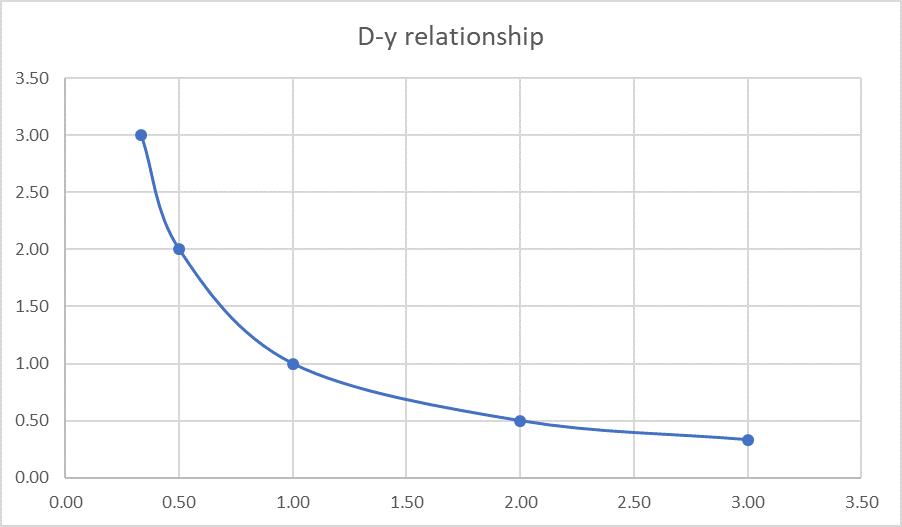
\includegraphics[width=16cm]{img//Newton.PNG}
\caption{牛顿迭代法}
\label{fig:sys.param}
\end{center}
\end{figure}

先根据市场年化率,猜测一个$y_1$,
对曲线上点$(y_1, D_1)$和$(y_0, D_0)$,我们可以求出$Duration = dp/dy$,
逐步调整$y_1$的值,缩小$\Delta y$,
把猜测的值往真实值逼近,
也就是牛顿迭代法。


%Chapter 6
\newpage
\section{实验结果}
<<<<<<< HEAD
\subsection{计算逻辑准确性测试}
Figure\ref{fig:sys.param}展示了测试计算逻辑模块的准确性时,系统输出的结果。
\begin{figure}[H]
\begin{center}
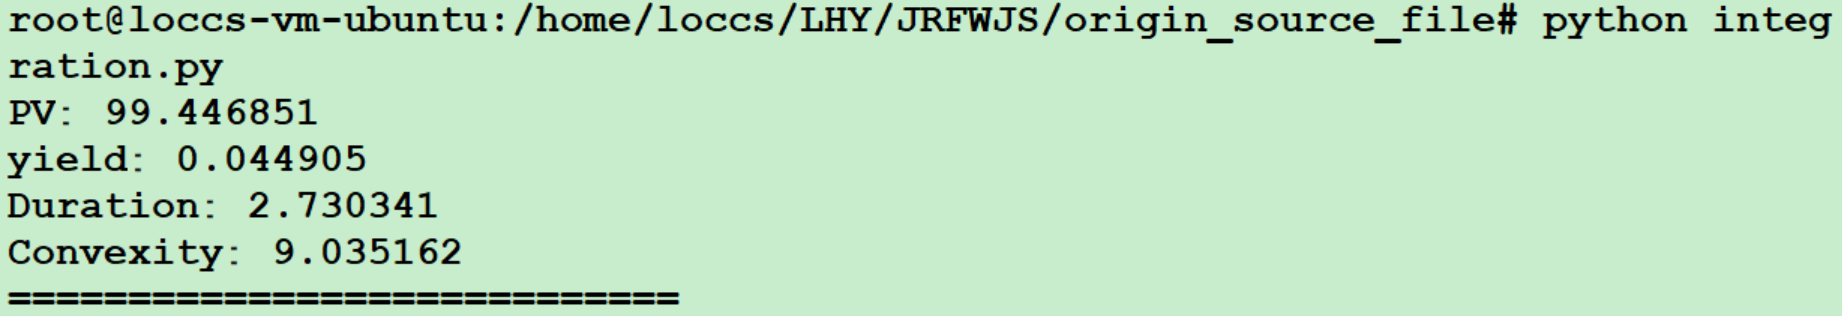
\includegraphics[width=16cm]{img//integration.PNG}
\caption{计算逻辑准确性测试}
\label{fig:sys.param}
\end{center}
\end{figure}
=======
输入:给定任意一个coupon bond
输出:该coupon bond的present value, duration以及convexity
	从市场获得与当前coupon bond相似的其他bond的y,这里的相似主要指的是利率、到期时间等相似
	通过牛顿迭代法找到需要的$y_i$,具体进行几轮牛顿迭代法,找到几个$y_i$,取决于从当前时刻到到期,还要发放利息几次
	利用上文给出的公式,将$y_i$的具体值带入,求出PV,duration和convexity。
>>>>>>> 66b0201b7af9b5681b33619e791efa5e5a4517e8


\subsection{自动测试结果}
Figure\ref{fig:sys.param}展示了使用自动测试程序测试本系统的准确性和性能时,自动测试程序输出的结果。
\begin{figure}[H]
\begin{center}
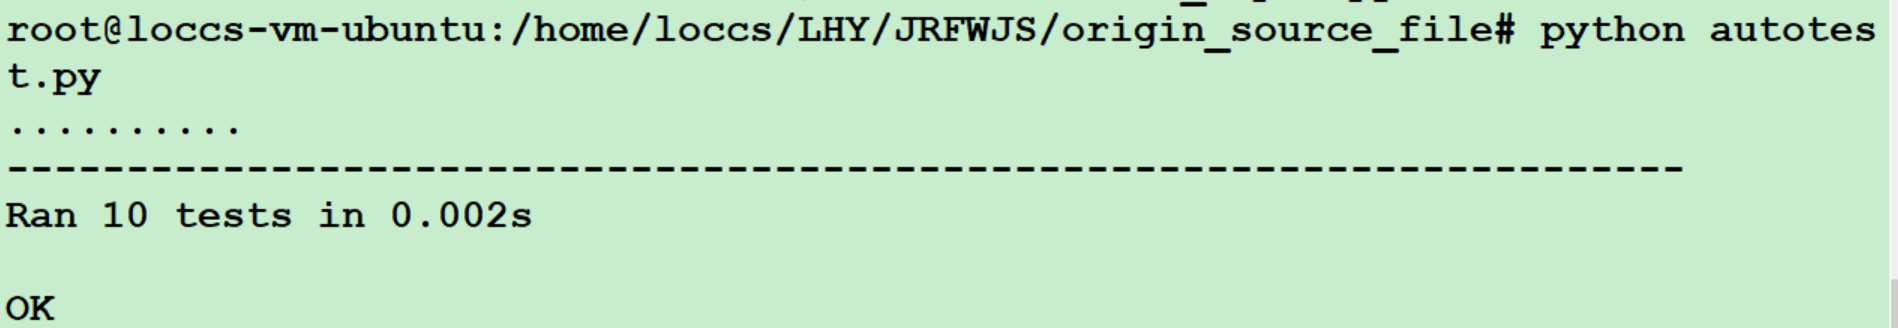
\includegraphics[width=16cm]{img//autotest.PNG}
\caption{自动测试结果}
\label{fig:sys.param}
\end{center}
\end{figure}


\subsection{调用多进程性能测试}
Figure\ref{fig:sys.param}展示了调用Python多进程时,系统输出的结果。
\begin{figure}[H]
\begin{center}
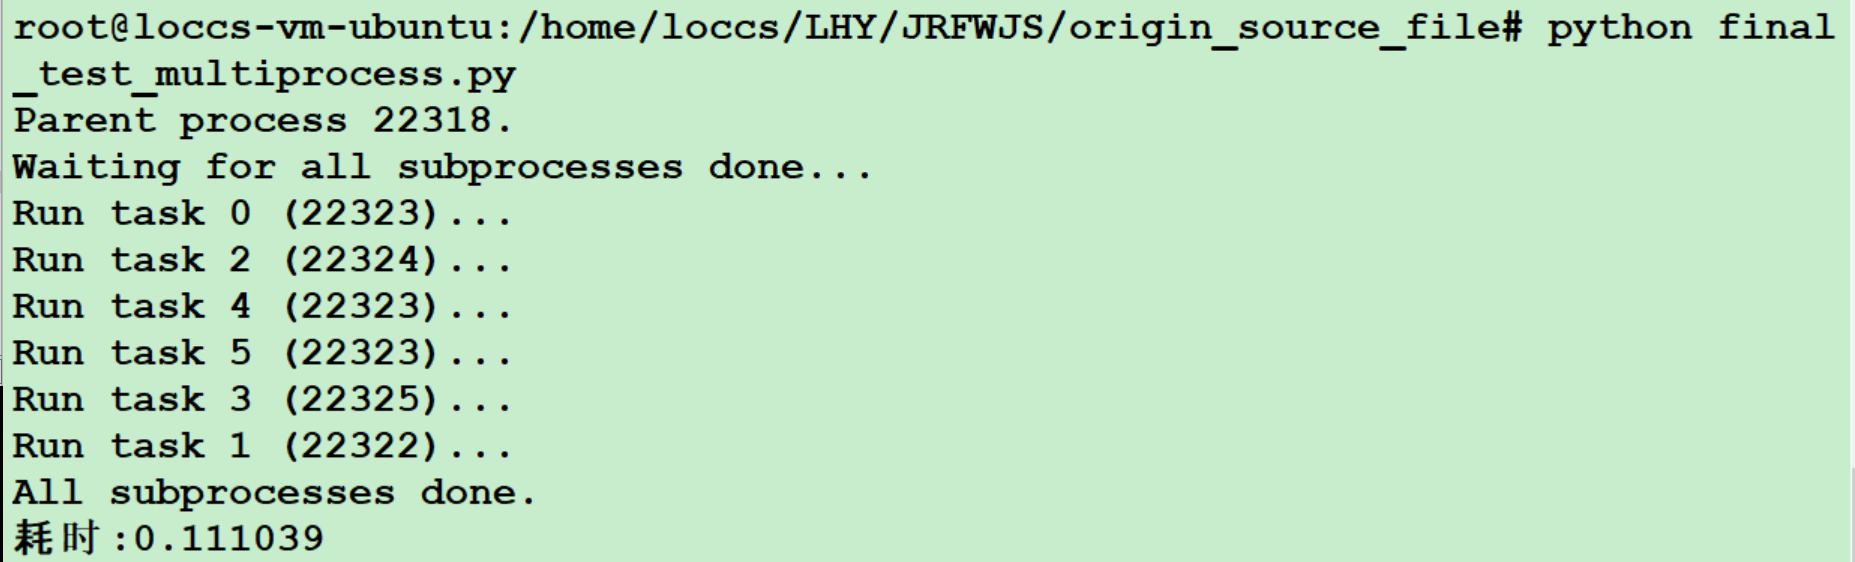
\includegraphics[width=16cm]{img//final_test_multiprocess.PNG}
\caption{调用多进程性能测试}
\label{fig:sys.param}
\end{center}
\end{figure}


\subsection{不使用并行计算}
Figure\ref{fig:sys.param}展示了不使用并行计算,运行用时103秒。
\begin{figure}[H]
\begin{center}
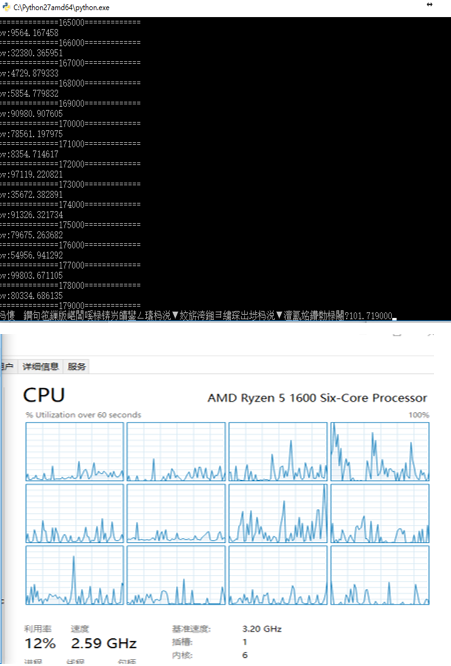
\includegraphics[width=16cm]{img//non_parallel.PNG}
\caption{不使用并行计算}
\label{fig:sys.param}
\end{center}
\end{figure}

\subsection{单机下并行计算}
Figure\ref{fig:sys.param}展示了单机并行百万级数据效果,用时11.83秒,效果不理想,因为文件io阻塞。
\begin{figure}[H]
\begin{center}
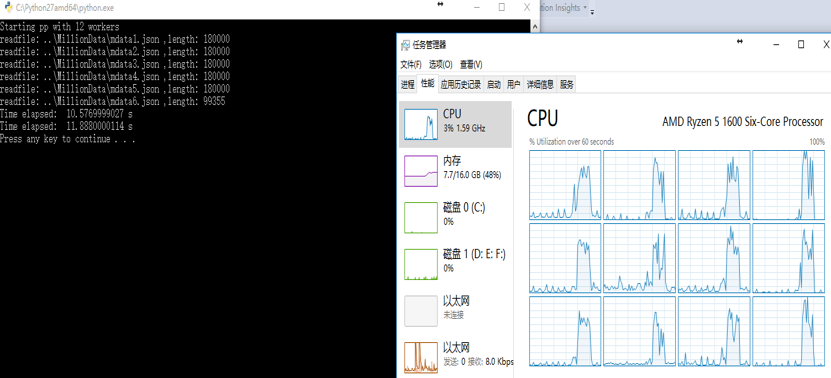
\includegraphics[width=16cm]{img//single_parallel.PNG}
\caption{单机下并行计算}
\label{fig:sys.param}
\end{center}
\end{figure}


\subsection{单机下并行计算的优化}
Figure\ref{fig:sys.param}展示了经过优化的单机并行百万级数据效果,用时10.63秒。
\begin{figure}[H]
\begin{center}
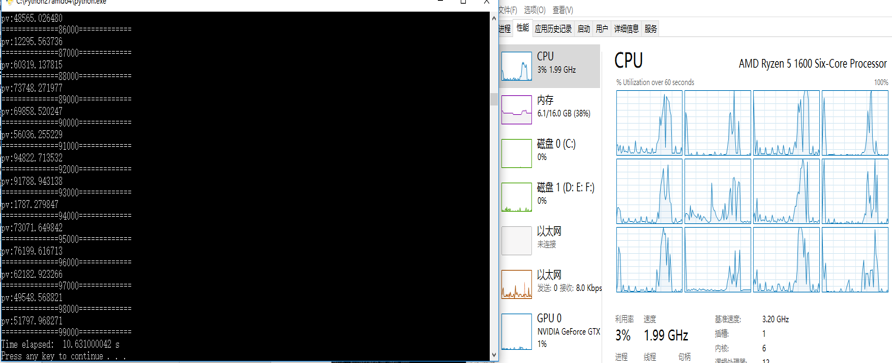
\includegraphics[width=16cm]{img//single_parallel_opt.PNG}
\caption{单机下并行计算的优化}
\label{fig:sys.param}
\end{center}
\end{figure}

\subsection{三百万数据测试}
Figure\ref{fig:sys.param}展示了三百万数据集下的测试结果。
\begin{figure}[H]
\begin{center}
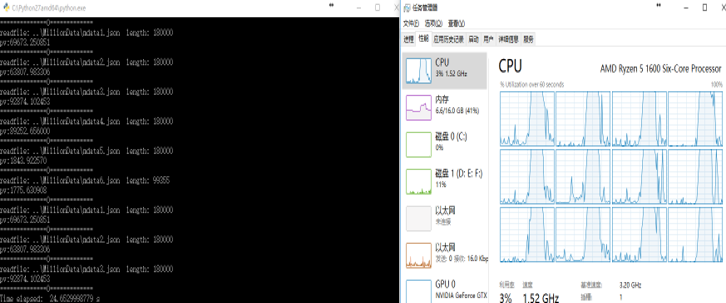
\includegraphics[width=16cm]{img//3million.PNG}
\caption{三百万数据测试}
\label{fig:sys.param}
\end{center}
\end{figure}

\subsection{分布式计算测试结果}
Figure\ref{fig:sys.param}展示了使用台式机+笔记本构成的集群下的测试结果。
\begin{figure}[H]
\begin{center}
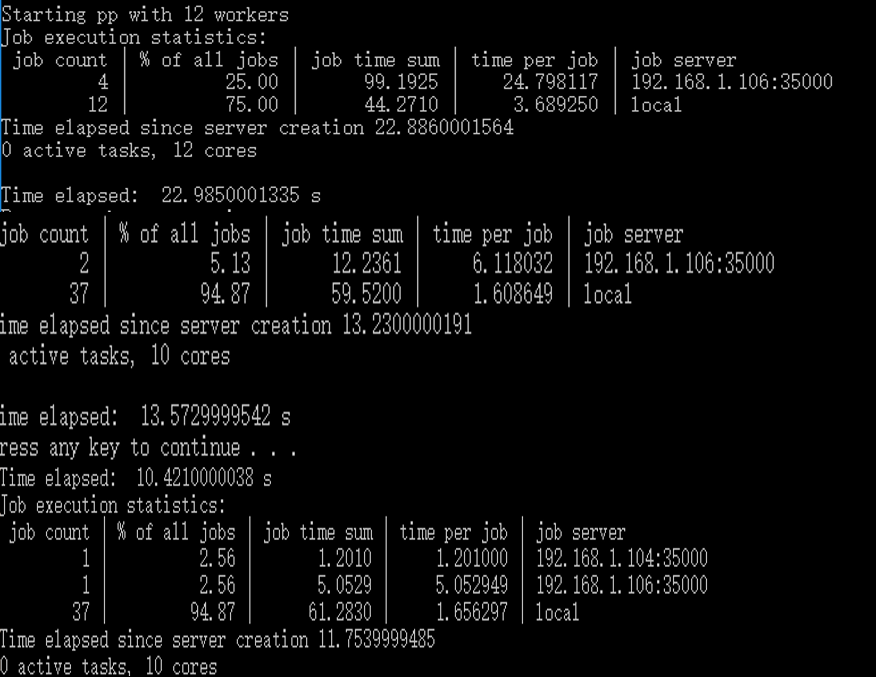
\includegraphics[width=16cm]{img//distribution.PNG}
\caption{分布式计算测试结果}
\label{fig:sys.param}
\end{center}
\end{figure}

%Chapter 7
\newpage
\section{界面展示}
\subsection{计算模块}

\paragraph{autotest} 
该子模块负责自动测试。
\begin{table}[H]
\begin{adjustwidth}{-3cm}{-3cm}
\begin{center}
\begin{tabular}{|p{.2\textwidth}| p{.8\textwidth}|} \hline
输入 & 无  \\ \hline
输出 & 运行测试集的数目,运行测试集所需时间  \\ \hline
描述 & 首先将一些测试用例写入Json文件,在该子模块中批量调用Json文件中的数据,将本模型的计算结果与测试集的正确结果进行比较,如果误差在允许范围内,认为该测试集运行通过,否则失败。  \\ \hline
\end{tabular}
\end{center}
\end{adjustwidth}
\end{table}


\paragraph{draw}
该子模块负责图片绘制。
\begin{table}[H]
\begin{adjustwidth}{-3cm}{-3cm}
\begin{center}
\begin{tabular}{|p{.2\textwidth}| p{.8\textwidth}|} \hline
输入 & 到期时间,计算收益的时间  \\ \hline
输出 & 时间与到期收益率的关系图 \\ \hline
描述 & 绘制时间与到期收益率的关系图。 \\ \hline
\end{tabular}
\end{center}
\end{adjustwidth}
\end{table}


\paragraph{final$\_$test$\_$multiprocess}
该子模块计算多进程使用的时间。
\begin{table}[H]
\begin{adjustwidth}{-3cm}{-3cm}
\begin{center}
\begin{tabular}{|p{.2\textwidth}| p{.8\textwidth}|} \hline
输入 & 无  \\ \hline
输出 & 调用多进程比直接运行父进程,所多花的时间 \\ \hline
描述 & 调用6个子进程,计算其运行所需的时间,将其与直接运行父进程所需的时间,进行对比。 \\ \hline
\end{tabular}
\end{center}
\end{adjustwidth}
\end{table}


\paragraph{final$\_$test$\_$singleprocess}
直接运行百万数据集的测试用例,所需的时间。
\begin{table}[H]
\begin{adjustwidth}{-3cm}{-3cm}
\begin{center}
\begin{tabular}{|p{.2\textwidth}| p{.8\textwidth}|} \hline
输入 & 无  \\ \hline
输出 & 在百万数据集上,调用多进程比直接运行父进程,多花的时间 \\ \hline
描述 & 在百万数据集上,调用7个子进程,计算其运行所需的时间,将其与直接运行父进程所需的时间,进行对比。 \\ \hline
\end{tabular}
\end{center}
\end{adjustwidth}
\end{table}


\paragraph{integration}
根据历史债券信息,计算债券在任意时刻的现值pv,其预计的综合年化收益率,久期和凸性。
\begin{table}[H]
\begin{adjustwidth}{-3cm}{-3cm}
\begin{center}
\begin{tabular}{|p{.2\textwidth}| p{.8\textwidth}|} \hline
输入 & 债券利率,债券本金,债券发行日期,债券年限,债券出售日期,债券付息频率  \\ \hline
输出 & 债券现值,到期收益率,久期,凸性 \\ \hline
描述 & 该子模块通过调用其他计算子模块,计算给定的任意债券的债券现值,到期收益率,久期,凸性。 \\ \hline
\end{tabular}
\end{center}
\end{adjustwidth}
\end{table}

\paragraph{LargeDataCalc}
读取json文件中的数据,进行批量处理。
\begin{table}[H]
\begin{adjustwidth}{-3cm}{-3cm}
\begin{center}
\begin{tabular}{|p{.2\textwidth}| p{.8\textwidth}|} \hline
输入 & Json文件  \\ \hline
输出 & Json文件 \\ \hline
描述 & 该子模块对大数据进行批量处理,从Json文件批量读取数据,再进行批量计算,将计算结果写入Json文件,并保存在本地。 \\ \hline
\end{tabular}
\end{center}
\end{adjustwidth}
\end{table}


\paragraph{newton}
使用牛顿迭代法,估计出目标债券的到期收益率。
\begin{table}[H]
\begin{adjustwidth}{-3cm}{-3cm}
\begin{center}
\begin{tabular}{|p{.2\textwidth}| p{.8\textwidth}|} \hline
输入 & 债券的当前价格,利率,本金,剩余付息次数,到下一次付息的时间/两次付息间隔,估计的精度,付息频率  \\ \hline
输出 & 估计的到期收益率 \\ \hline
描述 & 该子模块利用牛顿迭代法对给定债券在某时刻的到期收益率进行估计。 \\ \hline
\end{tabular}
\end{center}
\end{adjustwidth}
\end{table}


\paragraph{SQL}
连接SQL数据库。
\begin{table}[H]
\begin{adjustwidth}{-3cm}{-3cm}
\begin{center}
\begin{tabular}{|p{.2\textwidth}| p{.8\textwidth}|} \hline
输入 & 无  \\ \hline
输出 & 无 \\ \hline
描述 & 该子模块用于连接SQL数据库。 \\ \hline
\end{tabular}
\end{center}
\end{adjustwidth}
\end{table}


\paragraph{syield}
找到与给定债券相似的债券的到期收益率。
\begin{table}[H]
\begin{adjustwidth}{-3cm}{-3cm}
\begin{center}
\begin{tabular}{|p{.2\textwidth}| p{.8\textwidth}|} \hline
输入 & 给定债券的年限,给定债券剩下的付息次数,给定债券的到期时间,给定债券的付息频率,给定债券的发行日期  \\ \hline
输出 & 与给定债券相似的债券的到期收益率 \\ \hline
描述 & 该子模块通过在市场上寻找与给定债券的年限、付息次数、到期时间、付息频率、发行日期等参数相似的债券聚类,来得到估计的到期收益率。 \\ \hline
\end{tabular}
\end{center}
\end{adjustwidth}
\end{table}


\paragraph{time$\_$input}
时间输入程序,不考虑闰年的情况,每年都按365天计算。
\begin{table}[H]
\begin{adjustwidth}{-3cm}{-3cm}
\begin{center}
\begin{tabular}{|p{.2\textwidth}| p{.8\textwidth}|} \hline
输入 & 债券开始的时间,债券的年限,当前的时间,债券的付息频率  \\ \hline
输出 & 债券剩下的付息次数,距离下次发息时间,债券开始时间,债券结束时间 \\ \hline
描述 &  该子模块对于用户输入的时间进行标准化处理,将标准化的输出用于之后的子模块输入中。\\ \hline
\end{tabular}
\end{center}
\end{adjustwidth}
\end{table}


\subsection{加速模块}
\paragraph{C-Version-without static variables}
使用Cython编译各函数。

\paragraph{C-Version-static variables}
使用Cython编译各函数并使用静态变量。


\subsection{前端模块}
\paragraph{cover}
该子模块用于展示首页索引。

\paragraph{layout}
该子模块用于展示网页布局。

\paragraph{page1}
该子模块用于展示计算页面。

\paragraph{page2}
该子模块用于展示计算页面。

\paragraph{page3}
该子模块用于展示计算页面。

\paragraph{welcome}
该子模块用于展示欢迎页面。

\subsection{数据集}
我们提供了100万组债券的信息,用于测试本系统在大数据情况下的性能。通过调用C++加速、调用Python多进程、使用静态变量等本地加速和分布式计算的方式,来提高系统的处理速度。

%Chapter 8
\newpage
\section{组员分工}
\subsection{实验环境}
\paragraph{系统} Ubuntu 16.04.3 LTS
\paragraph{CPU} Intel Core5

\subsection{实验结果}
\paragraph{计算逻辑准确性测试}
图\ref{fig:sys.param}展示了测试计算逻辑模块的准确性时,系统输出的结果。
\begin{figure}[H]
\begin{center}
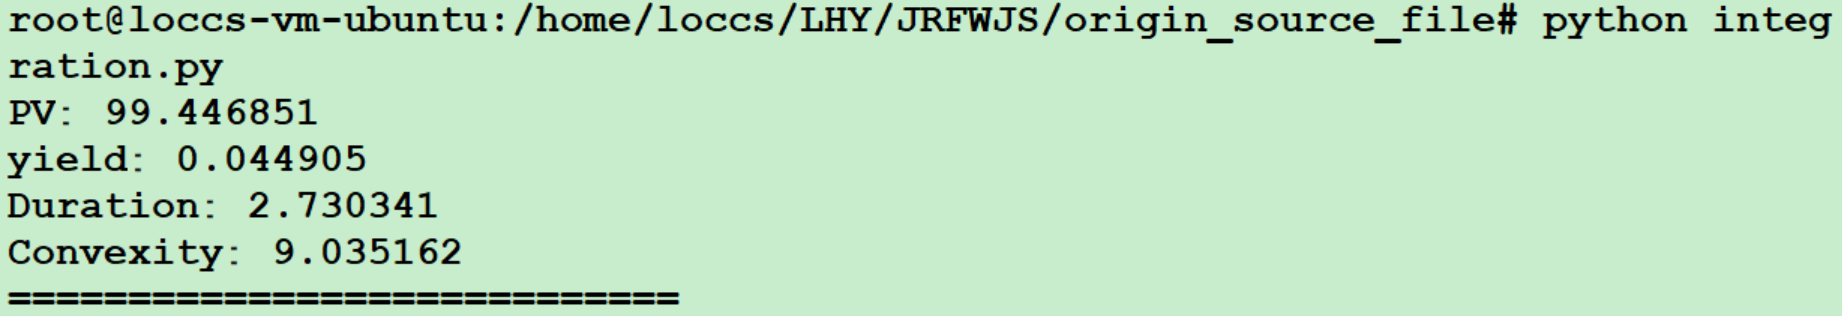
\includegraphics[width=16cm]{img//integration.PNG}
\caption{计算逻辑准确性测试}
\label{fig:sys.param}
\end{center}
\end{figure}


\paragraph{调用多进程性能测试}
图\ref{fig:sys.param}展示了调用Python多进程时,系统输出的结果。
\begin{figure}[H]
\begin{center}
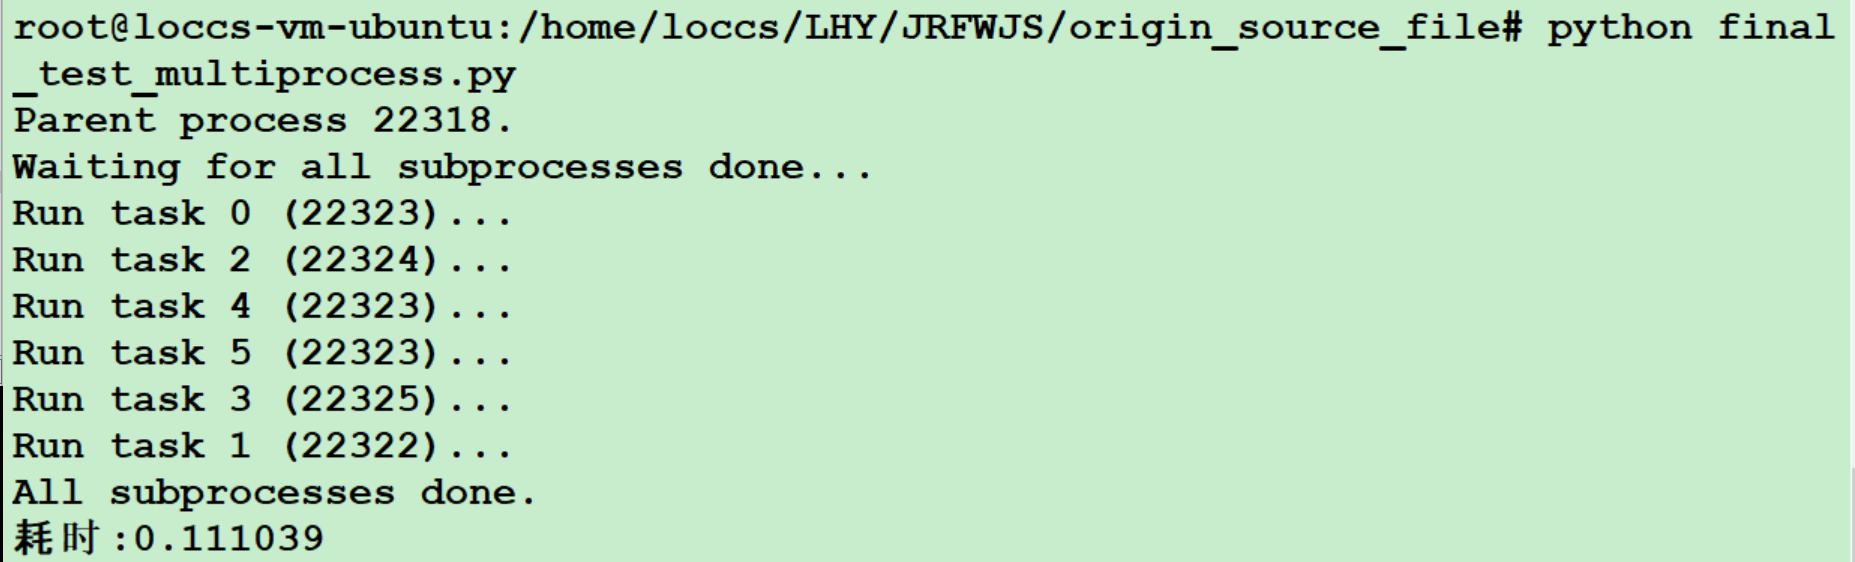
\includegraphics[width=16cm]{img//final_test_multiprocess.PNG}
\caption{调用多进程性能测试}
\label{fig:sys.param}
\end{center}
\end{figure}


\paragraph{自动测试结果}
图\ref{fig:sys.param}展示了使用自动测试程序测试本系统的准确性和性能时,自动测试程序输出的结果。
\begin{figure}[H]
\begin{center}
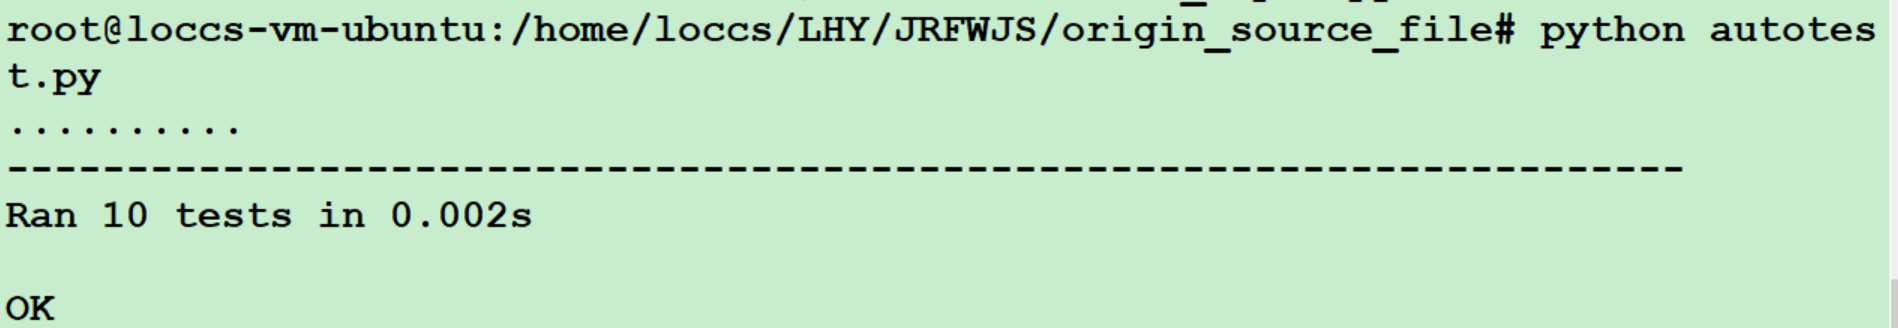
\includegraphics[width=16cm]{img//autotest.PNG}
\caption{自动测试结果}
\label{fig:sys.param}
\end{center}
\end{figure}


\paragraph{性能分析}在百万数据集上,调用C++加速。
\begin{table}[H]
\begin{adjustwidth}{-3cm}{-3cm}
\begin{center}
\begin{tabular}{|p{.8\textwidth}| p{.2\textwidth}|} \hline
技术手段 & 运行时间  \\ \hline
原始python代码 & 约50s  \\ \hline
使用Cython编译各函数 & 约38s  \\ \hline
使用Cython编译各函数并使用静态变量 & 约26s \\ \hline
\end{tabular}
\end{center}
\end{adjustwidth}
\end{table}

\paragraph{性能分析}在百万数据集上,调用Python多进程。
\begin{table}[H]
\begin{adjustwidth}{-3cm}{-3cm}
\begin{center}
\begin{tabular}{|p{.6\textwidth}| p{.2\textwidth}|p{.2\textwidth}|} \hline
技术手段 & 单进程时间 & 多进程时间 \\ \hline
原始python代码 & 约50s  & 约13s\\ \hline
使用Cython编译各函数 & 约38s  & 约11s\\ \hline
使用Cython编译各函数并使用静态变量 & 约26s & 约7.8s\\ \hline
\end{tabular}
\end{center}
\end{adjustwidth}
\end{table}



%Chapter 9
\newpage
\section{参考文献}
待补充。


\bibliography{reference}
\bibliographystyle{alpha}


\end{CJK}
\end{document}
